\chapter{Laboratorio 6: \\Functional Verification}
\section{VHDL Testing}
\subsection{A given RCA}
Nella prima parte dell'esperienza di laboratorio viene fornito il \textit{Test Bench} di un \textit{Ripple Carry Adder}, contenente un errore.\\
Il Test Bench era diviso sostanzialmente in tre parti:
\begin{itemize}
	\item \textbf{Random Input Values}
	\item \textbf{Reference Architecture}
	\item \textbf{Assert Instructions}
\end{itemize}
All'interno del codice si può notare come una volta generat
\subsection{A more complex case}
Nella seconda parte di questo primo esercizio viene richiesto di verificare la correttezza di quattro versioni di un circuito \textit{incrementer$\&$comparator} presente in Figura \ref{pentium}.
\begin{figure}[!htb]
	\centering
	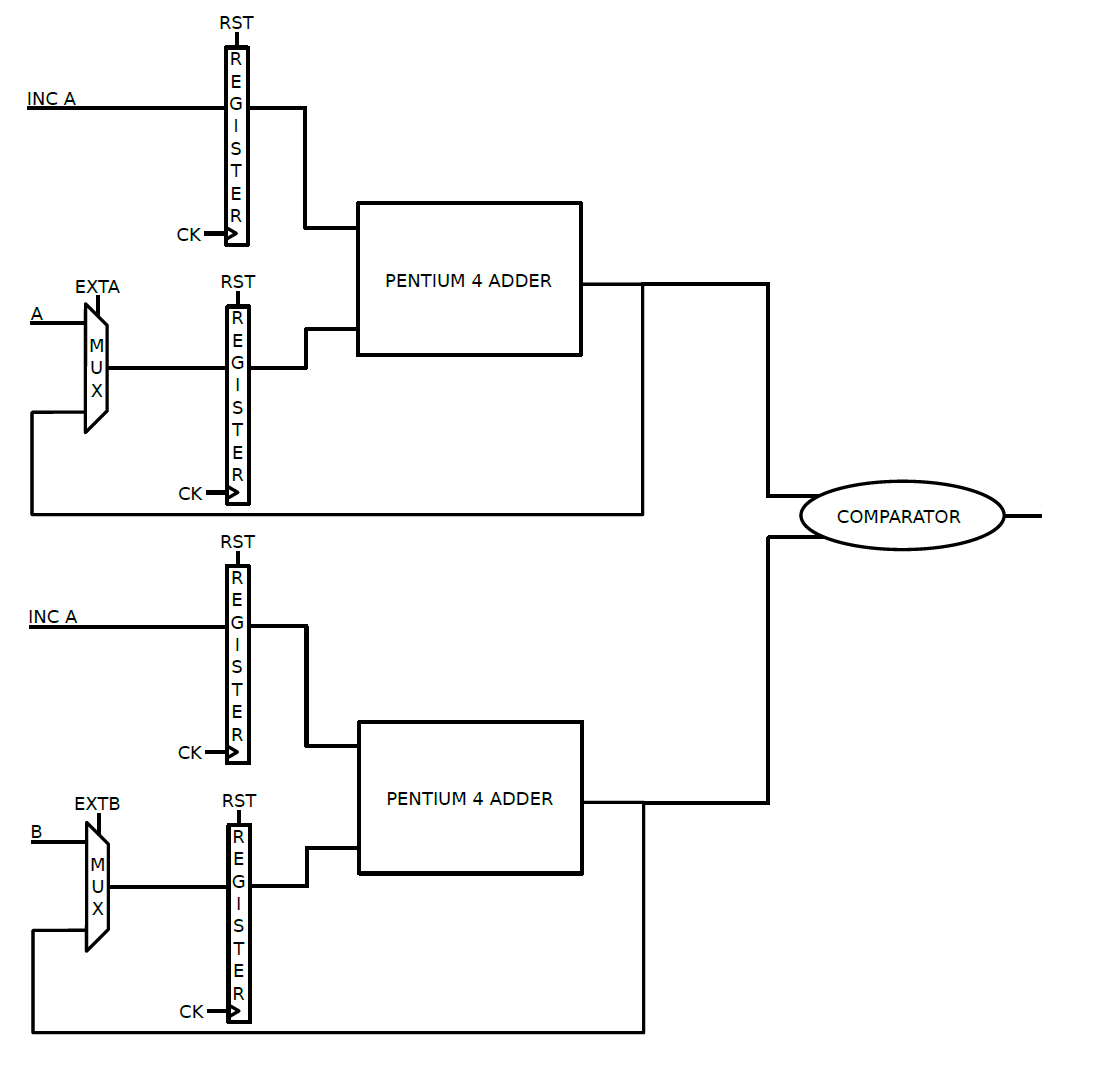
\includegraphics[scale=1]{immagini/pentium}
	\caption{\textit{Probabilità e Switching Activity stimati manualmente}}
	\label{pentium}
\end{figure}
La struttura presenta 4 blocchi diversi, replicati due volte, e un compatore:
\begin{itemize}
	\item  Due multiplexer a due vie che selezionano l'ingresso \textit{A} e \textit{B} oppure l'uscita del rispettivo sommatore con poi un Registro in uscita
	\item un registro per campionare l'ingresso \textit{INCA} e \textit{INCB} che decide se incrementare o meno l'ingresso A e B.
	\item due sommatori, realizzati tramite la struttura \textit{Pentium 4 Adder}
	\item un comparatore che manda in uscita il valore maggiore tra A e B
\end{itemize}
Dopo aver letto il funzionamento del Pentium 4 tramite l'appendice si è iniziata la realizzazione del TestBench per scoprire quali fossero i bug presenti. Veniva fornita una versione di riferimento del circuito, priva di bug in modo da avere un'architettura di riferimento con la quale confrontare le 4 versioni del circuito.\\
Il VHDL implementato per questo scopo è presente in Figura \ref{testbench_vhdl1} e \ref{testbench_vhdl2}.
\begin{figure}[!htb]
	\centering
	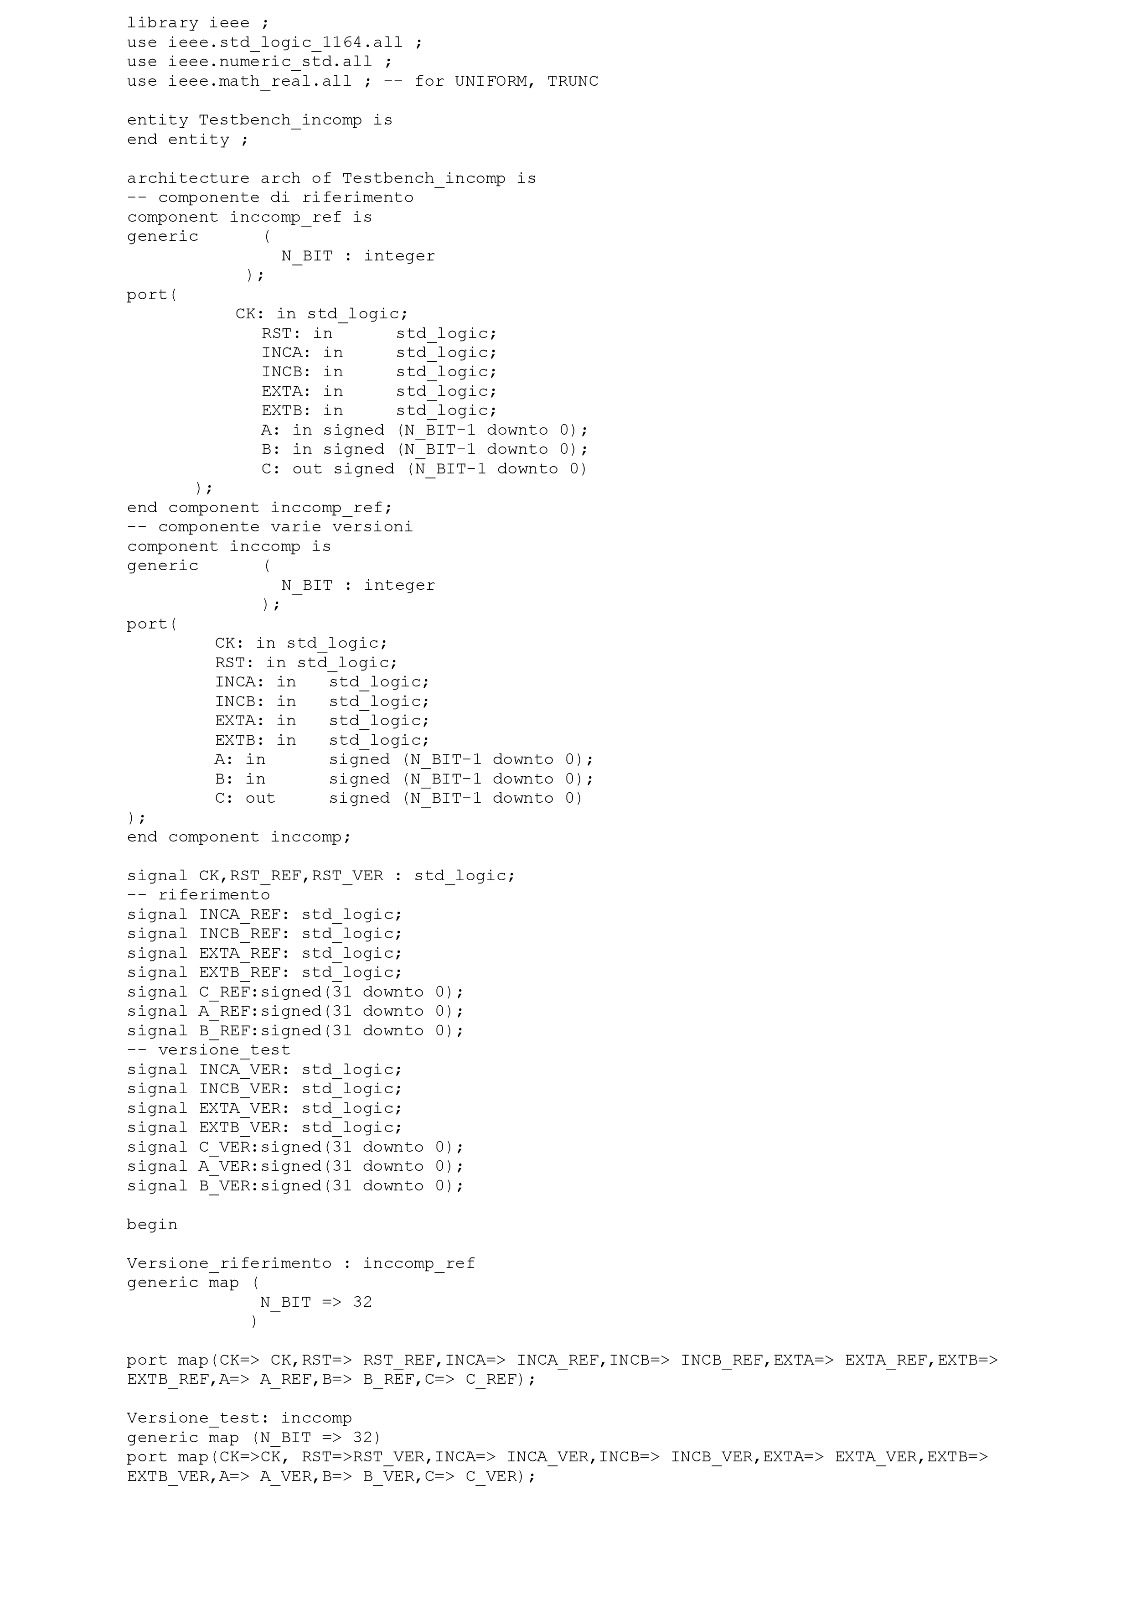
\includegraphics[scale=0.3]{immagini/testbench_vhdl1}
	\caption{\textit{Probabilità e Switching Activity stimati manualmente}}
	\label{testbench_vhdl1}
\end{figure}
\begin{figure}[!htb]
	\centering
	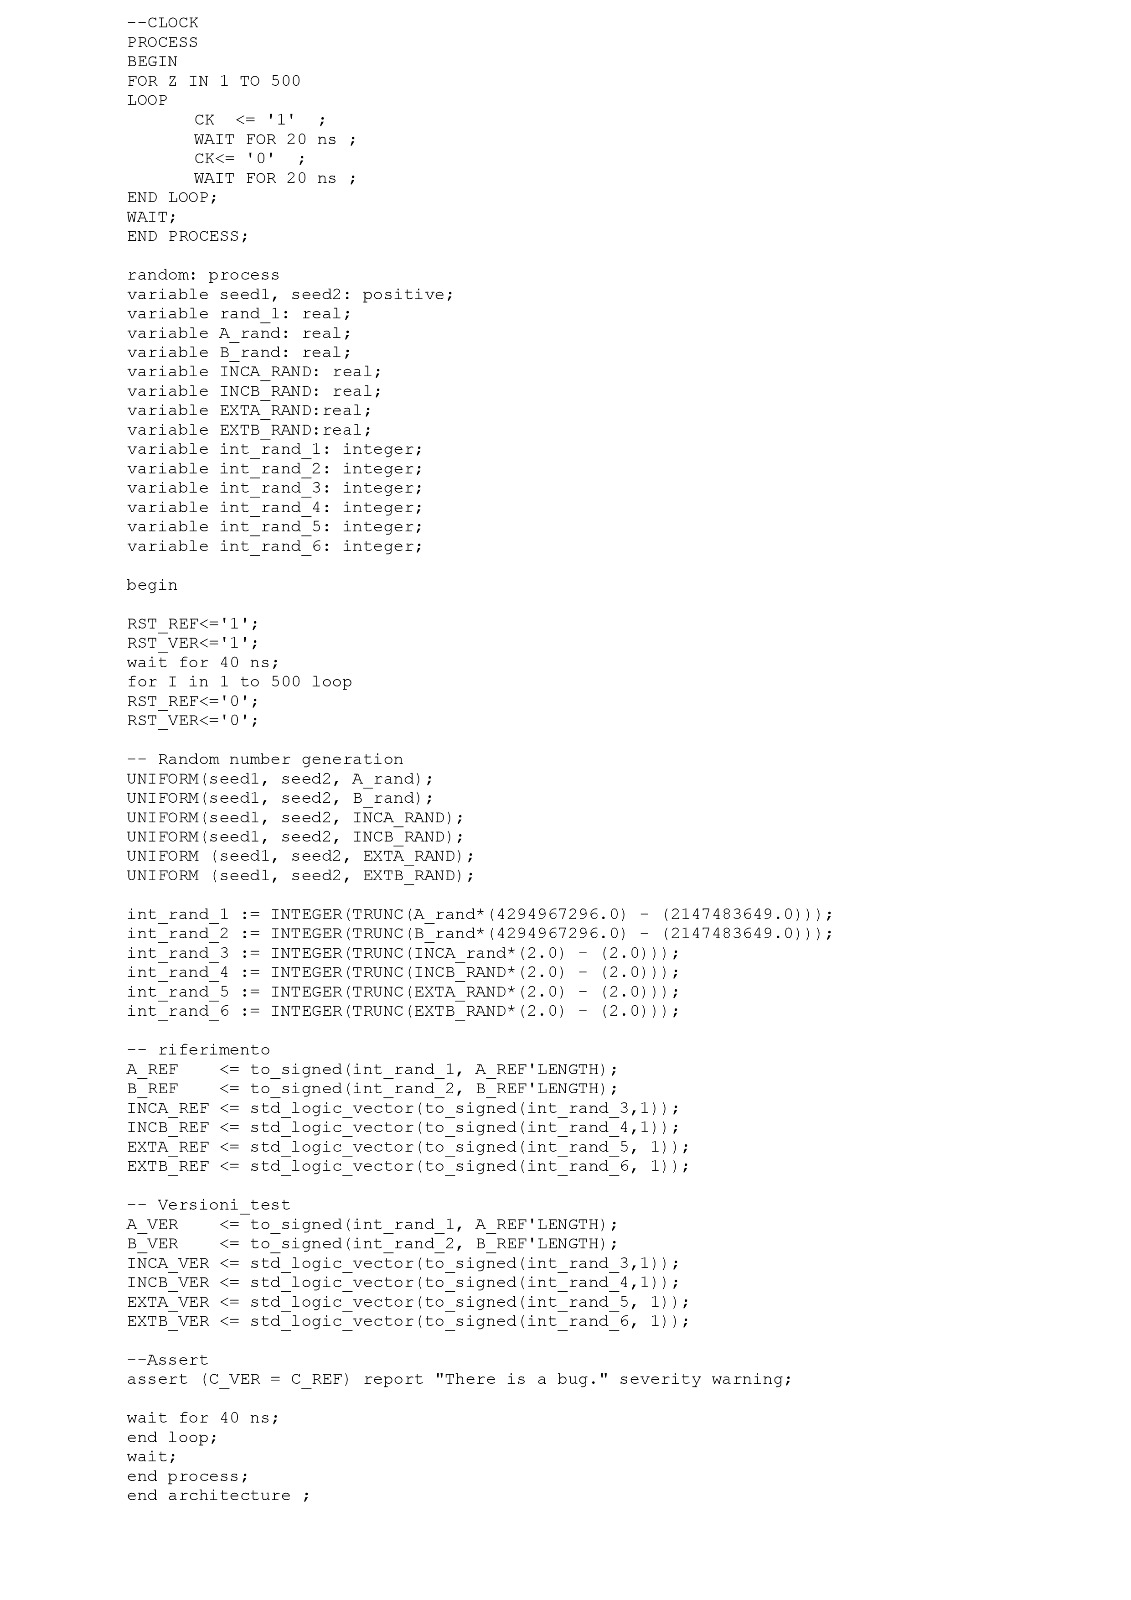
\includegraphics[scale=0.3]{immagini/testbench_vhdl2}
	\caption{\textit{Probabilità e Switching Activity stimati manualmente}}
	\label{testbench_vhdl2}
\end{figure}
\newpage
\noindent La struttura del Testbench è simile a quella fornita nell'esercizio precedente.\\
Ho una prima parte di generazione di numeri casuali, nello specifico genero in modo assolutamente randomico gli ingressi A e B, i selettori dei multiplexer EXTA e EXTB e gli ingressi di incremento INCA e INCB.\\
In realtà simulando attentamente il circuito ci si è resi conto di come la soluzione con numeri random non sia sempre ottimale per la ricerca di un bug, in quanto, specialmente nel caso di un ingresso con un numero di bit molto elevato, sono necessarie numerose iterazioni per provare tutte le possibili combinazioni. Questo sta alla base della mancato ritrovo del bug nella quarta versione, in quanto tramite un Testbench con numeri random non siamo riusciti a "sollecitare" l'errore: probabilmente si sarebbe dovuto studiare degli ingressi opportuni per sollecitare il sommatore in modo più specifico.\\
La seconda parte del TestBench prende gli ingressi sviluppati nella parte prima e genera le uscite sia dell'architettura di riferimento che della versione da analizzare.\\
Infine viene effettuato il confronto tra le due uscite e viene definita una funzione di \textit{assert} che fornisce sul \textit{Transcript} di Modelsim un messaggio di errore nel caso in cui venga rilevato un bug.
Nella prima versione del circuito risulta un errore all'interno di un multiplexer presente nel selettore di riporto del sommatore, in quanto l'ingresso riferito all' '1' e allo '0' risultavano invertiti. Questa prima versione ha un errore molto "visibile" e facile da trovare, sono state necessarie quindi pochissime iterazioni.\\
Nella seconda versione del circuito invece, risulta un errore nel selettore del multiplexer del sommatore, in quanto invece di assegnare
\begin{center}
	$C\_IN(N\_BIT/CARRY-1)$
\end{center} 
assegna 
\begin{center}
	$C\_IN(N\_BIT/CARRY-2)$
\end{center}
Per trovare quest'errore sono state necessarie 500000000 iterazioni, un numero già ritenuto eccessivo. Si riporta in allegato in Figura \ref{sim1} la simulazione Modelsim contenente l'errore.
\begin{figure}[!htb]
	\centering
	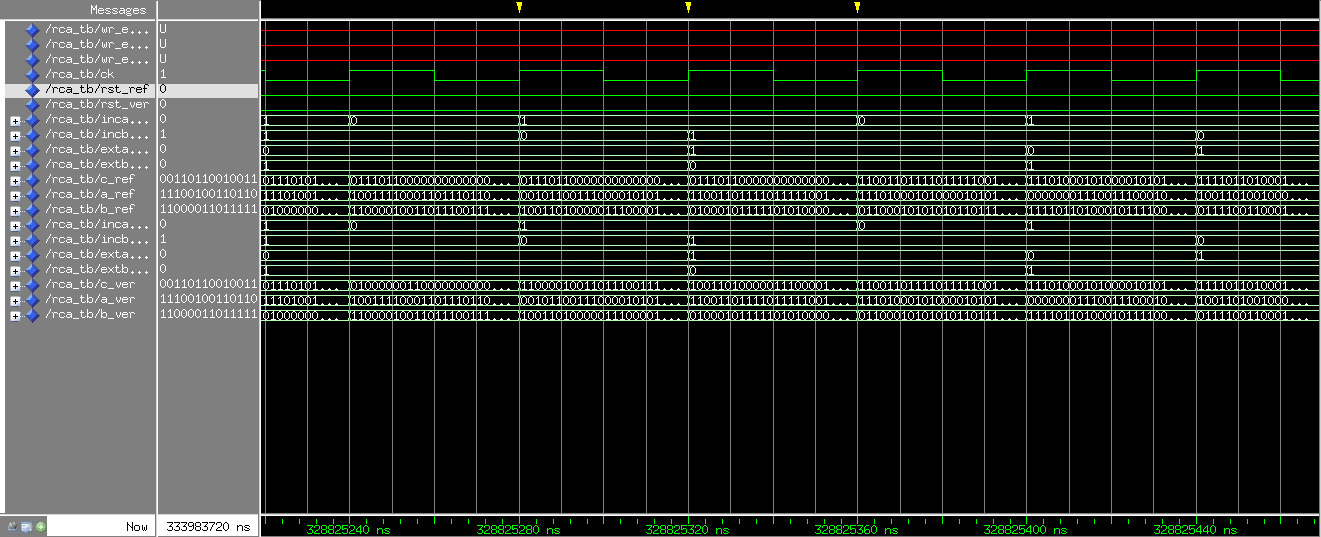
\includegraphics[scale=0.6]{immagini/sim1}
	\caption{\textit{Probabilità e Switching Activity stimati manualmente}}
	\label{sim1}
\end{figure}
\subsection{Finite State Machine}
Questa parte prevede di testare il  funzionamento di una FSM (Macchina a stati finiti), disponibile in 4 versioni differenti, contenenti dei bug.  
La FSM da testare è, un contatore up/down a 3 bit, la FSM è la seguente:
\begin{figure}[!htb]
	\centering
	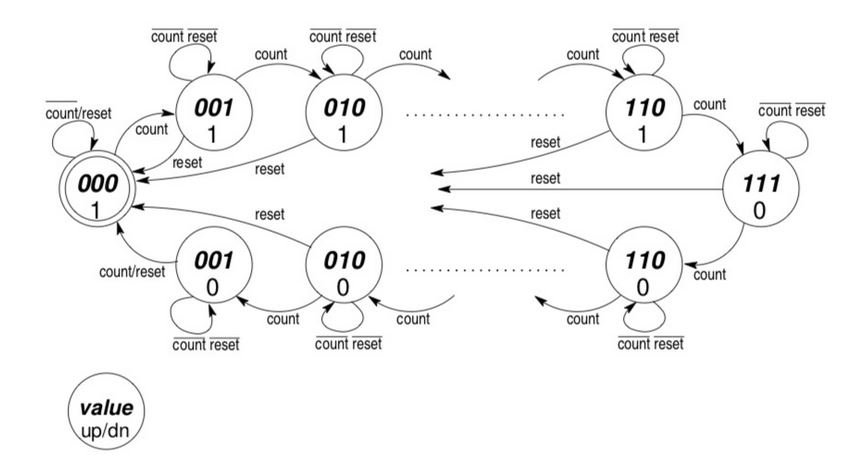
\includegraphics[scale=0.3]{immagini/fsm_lab6}
	\caption{\textit{Macchina a stati da testare}}
	\label{Fsm, up-down counter}
\end{figure}
\\
\\
\\
\\
\\
\\
\\
Prendendo spunto dal punto precedente il test è stato realizzato mediante i seguenti file:\\
counter\_ref.vhd, è il file del contatore dal corretto funzionamento, utilizzato per calcolare le uscite corrette da confrontare successivamente.
\\
counter.vhd, è il dispositivo da testare, disponibile in 4 versioni, site in diverse cartelle, poi estratte da modelsim volta per volta durante la simulazione
\\
counter\_tb.do, è lo script che si occupa di dirigere la compilazione e simulazione dei 4 files da testare su Modelsim, in cui è impostata anche la durata della simulazione e la visualizzazione delle forme d’onda dei segnali rilevanti ai fini della verifica, per consentire una comoda visione dell’andamento temporale dei segnali.
Di seguito un estratto del file disponibile in appendice.
\\
.......\\
.......\\
echo "testing v1..."\\
\\
vcom -reportprogress 300 -work work\\ /home/lp19.12/repository/lab6/ese6/3/counter\_tb.vhd\\ /home/lp19.12/repository/lab6/ese6/3/vREF/counter\_ref.vhd\\ /home/lp19.12/repository/lab6/ese6/3/v1/counter.vhd\\
\\
vsim -t ns -novopt work.counter\_tb\\
\\
set NumericStdNoWarnings 1\\
run 0 ps\\
set NumericStdNoWarnings 0\\
\\
add wave -radix binary   -color BLUE\\      sim:/counter\_tb/DATA\_OUT\_tb\\
add wave -radix binary   -color GREEN\\    sim:/counter\_tb/DATA\_OUT\_ref\\
add wave -radix binary   -color BLUE\\     sim:/counter\_tb/UP\_DN\_tb\\
add wave -radix binary   -color GREEN \\   sim:/counter\_tb/UP\_DN\_ref\\
run 30000000 ns\\
\\
echo "end v1"\\
.......\\
.......\\
\\


